\documentclass[12pt]{ociamthesis}  % default square logo 
%\documentclass[12pt,beltcrest]{ociamthesis} % use old belt crest logo
%\documentclass[12pt,shieldcrest]{ociamthesis} % use older shield crest logo

%load any additional packages
\usepackage{amssymb}
\usepackage{url}          % needed for \url{} in website citations
\usepackage{subcaption}   % needed for side-by-side figures via subfigure

%input macros (i.e. write your own macros file called mymacros.tex 
%and uncomment the next line)
%\include{mymacros}

\title{Design and Deployment of an
\\[1ex]Imaging Spectrometer for the
\\[1ex]Characterisation of Spatial Chirp
}   %note \\[1ex] is a line break in the title

\author{Ron Ellenbogen}             %your name
\college{Supervised by Dr. Benjamin Greenwood
\\[1ex]Laser Plasma Accelerator Group}  %your college

\renewcommand{\submittedtext}{Summer Research Project
\\[1ex]}
\degree{}     %the degree
\degreedate{August 2026}   %the degree date

%end the preamble and start the document
\begin{document}

%this baselineskip gives sufficient line spacing for an examiner to easily
%markup the thesis with comments
\baselineskip=18pt plus1pt

%set the number of sectioning levels that get number and appear in the contents
\setcounter{secnumdepth}{3}
\setcounter{tocdepth}{3}


\maketitle                  % create a title page from the preamble info

\begin{romanpages}          % start roman page numbering
\tableofcontents            % generate and include a table of contents
\listoffigures              % generate and include a list of figures
\end{romanpages}            % end roman page numbering

%now include the files of latex for each of the chapters etc
\chapter{Introduction}
\label{chap:introduction}

\section{{Plasma Modulated Plasma Accelerator}}
\label{sec:intro-motivation}
A plasma can be formed by ionising a gas target using a high-intensity, short (10 fs) laser pulse. 
The interaction of the laser pulse with the plasma can form accelerating structures with field 
strengths of the order of 100 GV/m. In a laser-wakefield accelerator scheme (LWFA), these accelerating structures may be used 
to achieve electron energies in the order of 100s MeV to GeV \cite{esarey2009}. Such schemes may lead to the production of compact, low cost
electron sources with applications such as light source generation \cite{geddes2017}, QED experiments \cite{los2025}, radiobiology studies
 \cite{mcanespie2024}, and probing fundamental plasma 
physics \cite{balcazar2025}.

LWFA schemes are currently limited by the repititon rates of their laser systems, most commonly $\lessapprox$ 10 Hz with Ti:sapphire lasers. 
The University of Oxford's Laser Plasma Accelerator Group (LPAG) is working with collaborators on the plasma-modulated plasma accelerator (P-MoPA)
project to address this \cite{jakobsson2021,alejo2022,vandewetering2023,vandewetering2024,ross2024}. The project aims to use thin-disk lasers
with high repititon rates ($\sim$ 1 kHz) to drive a LWFA electron source. The pulse duration of such lasers is too long too drive a LWFA, so
the following scheme is used to create a pulse-train (see Figure~\ref{fig:pmopa}): A short, low-energy seed-pulse is co-propagated with a long drive-pulse through
a modulator stage containing a gas. The seed-pulse ionises the gas and drives a low-intensity plasma wave that modulates the drive-pulse,
producing side-bands in its spectrum. A compressor then removes the phase on these side-bands, converting the picosecond pulse into a train
of short pulses spaced temporally by the plasma period. This pulse train can then be directed into a second plasma stage of the same density,
resonantly exciting a wakefield into which electrons can be injected and subsequently accelerated. This modulation-compression process is
sensitive to the drive-pulse's spatio-spectral content; any spatio-spectral couplings would vary the modulation across the pulse's profile and
degrade the resulting pulse-train, weakening the pulse-train's ability to drive a wakefield and leading to unstable electron acceleration.
The characterisation of spatio-spectral couplings in the thin-disk lasers used in the P-MoPA project is thus essential for the project's success.

\begin{figure}[tbp]
    \centering
    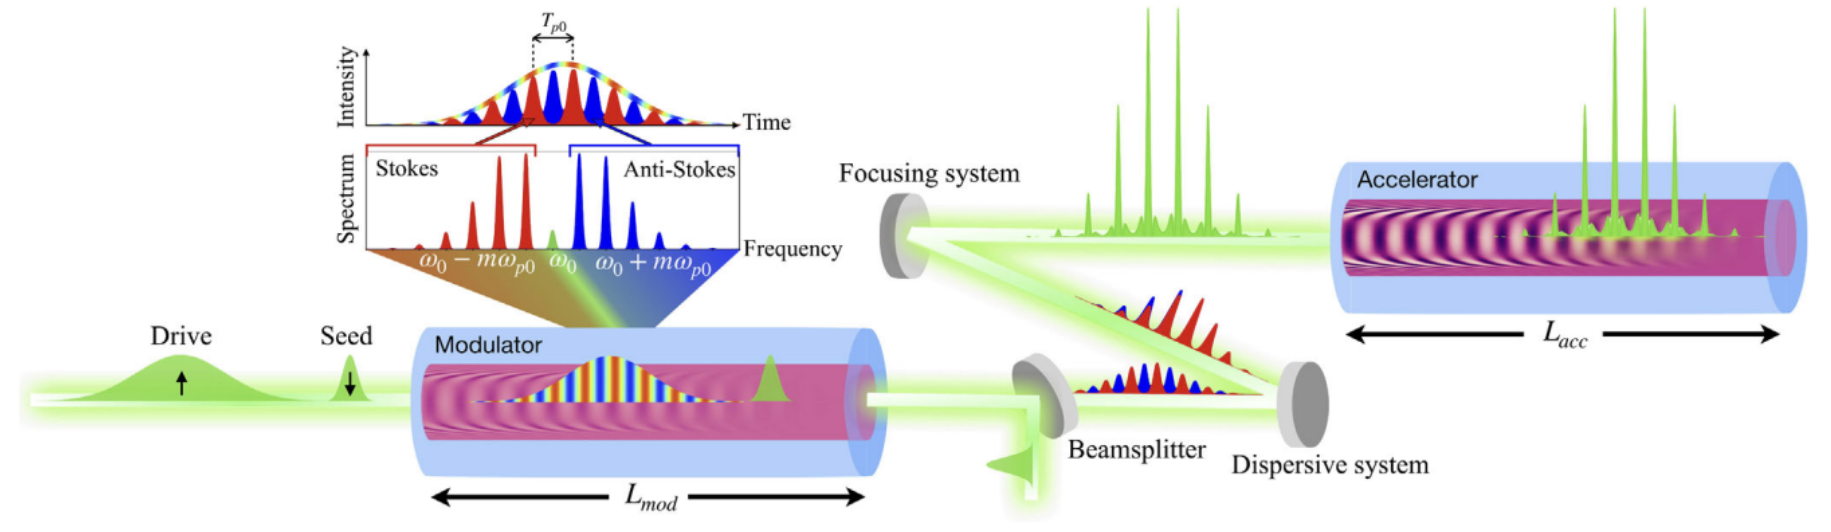
\includegraphics[width=\textwidth]{figures/pmopa.png}
    \caption[The Plasma Modulated Plasma Accelerator (P-MoPA) scheme.]{The Plasma Modulated Plasma Accelerator (P-MoPA) scheme. Reproduced from \cite{jakobsson2021}.}
    \label{fig:pmopa}
\end{figure}


\section{Angular and Spatial Chirp}
\label{sec:intro-background}

\subsection{Chirped Pulse Amplification}
\label{sec:intro-cpa}

Prior to Gérard Mourou and Donna Strickland's invention of chirped pulse
amplification (CPA) \cite{strickland1985}, for which they were awarded the Nobel Prize in Physics
in 2018, it was extremely challenging to produce ultrashort laser pulses with
enough intensity
for modern LWFA without damaging the optical equipment and introducing
non-linear effects. CPA avoids these issues through a staged amplification
procedure (see Figure~\ref{fig:cpa}): An ultrashort, low-amplitude pulse enters
a pulse stretcher, composed of two identical parallel diffraction gratings. 
This stretches the pulse temporally, reducing its intensity without loss of
energy. The pulse is subsequently amplified then directed through a pulse 
compressor, similar to the pulse stretcher, which compresses the pulse back to 
its original duration. The result is a high-intensity ultrashort pulse, but 
crucially this intensity is only reached post-compressor, leaving all previous
optical components unharmed.

As with most real optical systems, CPA systems are highly sensitive to
misalignments. In particular, a relative misalignment between the two gratings
of the stretcher or the compressor, or a mismatch between the dispersive properties
of the stretcher and the compressor, may produce spatio-spectral couplings in the 
pulse. One such coupling is known as \emph{angular chirp}, a correlation between 
the angle
of propagation $\theta$ and wavelength $\lambda$ within a pulse of finite bandwidth. 
When an angularly chirped pulse propagates over a finite distance, it acquires
\emph{spatial chirp}, a correlation between position $x$ along an arbitrary 
transverse axis across a pulse 
and wavelength $\lambda$.

\begin{figure}[tbp]
    \centering
    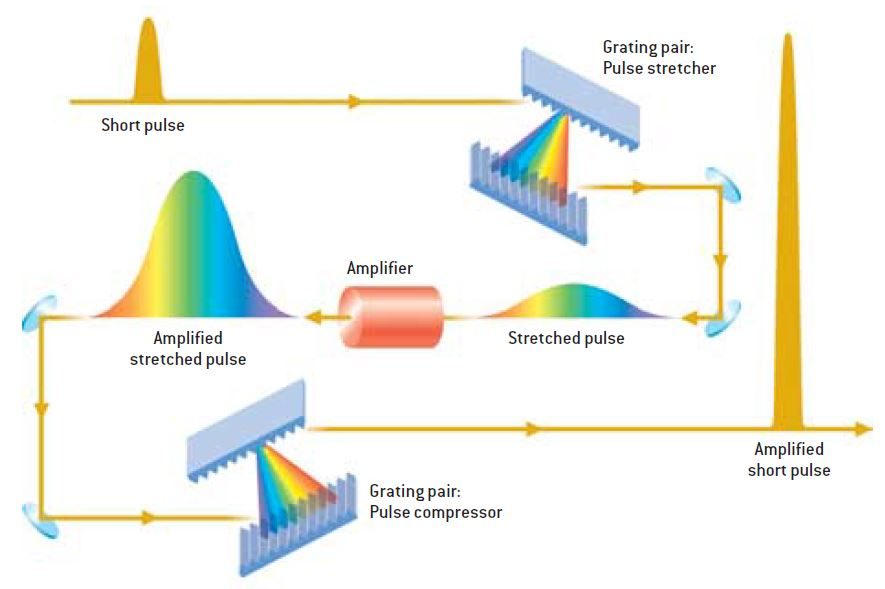
\includegraphics[width=\textwidth]{figures/CPA.jpg}
    \caption[Illustration of Chirped Pulse Amplification (CPA).]{Illustration of
     Chirped Pulse Amplification (CPA). Reproduced from \cite{cuos2026}.}
    \label{fig:cpa}
\end{figure}

% TODO: Brief CPA primer (stretch -> amplify -> compress) -- only as much as
% needed to motivate why the amplified pulse can pick up spatio-spectral
% coupling. See presentation slide 5.

\subsection{Angular-to-Spatial Chirp Conversion at Focus}
\label{sec:intro-angular-to-spatial}

\begin{figure}[tbp]
    \centering
    \begin{subfigure}[b]{0.48\textwidth}
        \centering
        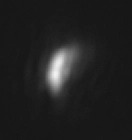
\includegraphics[width=\textwidth]{figures/lens_spatial_chirp.jpg}
        \caption{Lens focus}
        \label{fig:lens-focus}
    \end{subfigure}
    \hfill
    \begin{subfigure}[b]{0.48\textwidth}
        \centering
        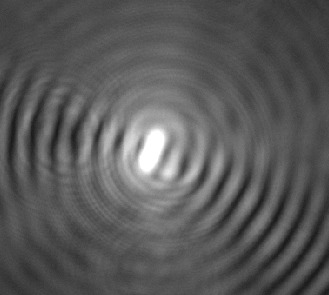
\includegraphics[width=\textwidth]{figures/axicon_spatial_chirp.jpg}
        \caption{Axicon focus}
        \label{fig:axicon-focus}
    \end{subfigure}
    \caption[Spatially chirped lens and axicon foci.]{
        Spatially chirped foci resulting from angularly
    chirped incident pulses. Images courtesy of Alexander Harrison.}
    \label{fig:lens_and_axicon_foci}
\end{figure}

A useful property of the converging lens is the conversion between angular and spatial
information at its focal plane. In particular, any collimated plane wave 
incident on an ideal thin lens of focal length $f$ is, in the paraxial 
approximation, focussed to a transverse position $x$ on the lens' 
back focal plane proportional to its angle of incidence $\theta$:
\begin{equation}
    x=f\theta.
    \label{eq:fourier_lens}
\end{equation}
Consequently, if the incident pulse is angularly chirped, 
meaning $\theta$ is spectrally dependent, the transverse position $x$ of the 
resulting focal spot
also becomes spectrally dependent, meaning it is spatially chirped. The result is 
a focal spot that is stretched along an arbitrary transverse axis, as
opposed to a typical circular focal spot. (see Figure
\ref{fig:lens_and_axicon_foci}).
 
Differentiating Equation \ref{eq:fourier_lens} with respect
to wavelength $\lambda$:
\begin{equation}
    \frac{dx}{d\lambda}=f\frac{d\theta}{d\lambda}.
    \label{eq:ang_to_spat_chirp}
\end{equation}
The derivative $\zeta\equiv\frac{dx}{d\lambda}$ is known as \emph{spatial dispersion},
corresponding to a pulse's spectrally dependent transverse position $x(\lambda)$, and
is the conventional metric used for describing spatial chirp throughout this 
project. Another common metric used for describing spatial chirp is known as 
the frequency gradient, $\frac{d\omega}{dx}$, corresponding to a pulse's 
transverse-positionally dependent angular frequency $\omega(x)$. While these
parametarisations both describe spatial chirp, they are not simply reciprocals of
each other \cite{gu2004}. Spatial dispersion is used throughout this project because
of its convenient relationship with the angular dispersion $\frac{d\theta}{d\lambda}$
that produces it. Wavelength is chosen as the spectral unit throughout this project
due to its direct relationship with the diffraction angle of optical gratings.



% TODO: Derive/explain how angular chirp d(theta)/d(lambda) upstream of a
% focussing optic becomes spatial chirp dx/d(lambda) at focus. See
% presentation slides 6-7 (lens vs axicon focus comparison).

\subsection{Consequences for the Plasma Wave}
\label{sec:intro-consequences}

% TODO: Spatial chirp -> elongated focal spot / longer pulse duration /
% reduced intensity; angular chirp -> pulse front tilt -> asymmetric drive
% of the plasma wave. See presentation slide 8 ("Why Should You Care?").

\section{Measuring Angular Chirp}
\label{sec:intro-measuring}

% TODO: Motivate the imaging-spectrometer approach as the measurement
% technique chosen (transition from "how do we measure this" to "here is
% the instrument we built" -- bridges into chapter 2). See presentation
% slide 9.

\section{Project Objectives}
\label{sec:intro-objectives}

% TODO: State the concrete goals -- design and deploy an imaging
% spectrometer, build the acquisition/calibration/preprocessing/analysis
% software pipeline, build a GUI, and use it to test a known spatial-chirp
% source (glass windows).

\section{Report Outline}
\label{sec:intro-outline}

% TODO: One short paragraph per remaining chapter (Optical Design,
% Calibration, Analysis Pipeline, Graphical User Interface, Experimental
% Design, Results, Discussion, Conclusions).
   % Introduction
\chapter{Optical Design}
\label{chap:optical-design}

\section{Design Requirements}
\label{sec:optical-requirements}

% TODO: What the instrument needed to do (resolve spatial position along a
% vertical entrance slit vs wavelength, fit in the available bench space,
% work with the existing Ti:sapphire beam) and the constraints that shaped
% the choices below.

\section{4f All-Transmissive Layout vs Czerny-Turner}
\label{sec:optical-layout-choice}

% TODO: Why a 4f all-transmissive design (transmission grating, achromatic
% doublets) was chosen over a Czerny-Turner (mirror-based) layout --
% simpler geometry, less astigmatism-prone, less chromatic-aberration-prone.
% See presentation slide 18 for the comparison figure.

\section{Optical Layout}
\label{sec:optical-layout}

% TODO: Walk through the beam path: vertical entrance slit -> collimating
% lens (achromatic doublet) -> transmission grating -> plane mirrors ->
% focussing lens (achromatic doublet) -> plane mirrors -> 90-degree
% periscope -> camera. See presentation slides 11-12 (schematic + bench
% photo) and slide 17 (periscope geometry) -- the periscope may warrant its
% own subsection if the geometry needs deriving in detail.

\section{Camera and Acquisition Hardware}
\label{sec:optical-camera}

% TODO: Basler a2A1920-51gmBAS via pypylon -- sensor format, pixel format,
% canonical frame shape/dtype (see src/pipeline/acquisition/frame.py and
% configs/default.yaml), and how CameraStream's background-thread
% acquisition model fits into the optical design (i.e. why this section
% belongs here rather than in the Analysis Pipeline chapter).

\section{Alignment Procedure}
\label{sec:optical-alignment}

\subsection{Grating-Camera Axis Alignment}
\label{sec:optical-grating-camera-alignment}

% TODO: What "grating-camera axis misalignment" looks like on a raw frame
% and how it was corrected. See presentation slide 19 (misaligned vs
% corrected spectral-line images).

\subsection{Slit-Camera Axis Alignment}
\label{sec:optical-slit-camera-alignment}

% TODO: Same for slit-camera axis alignment. See presentation slides 20-22
% (misaligned vs corrected images with fitted alignment lines).
   % Optical Design
\chapter{Calibration}
\label{chap:calibration}

\section{Calibration Architecture}
\label{sec:calib-architecture}

% TODO: The build/apply split -- calibration/ builds artifacts,
% preprocessing/ applies them -- and why that separation exists (a science
% frame's settings are checked against the artifact's recorded
% exposure/gain/timestamp via CalibrationRecord before it's applied). Frame
% this as the organizing principle for the rest of the chapter.

\section{Sensor Calibration}
\label{sec:calib-sensor}

\subsection{Baseline}
\label{sec:calib-baseline}

% TODO: Per-session background/dark average; background_sigma measured for
% free from the same stacked frames, used later in the noise model
% (chapter 4).

\subsection{Flat Field}
\label{sec:calib-flat-field}

% TODO: PRNU correction from uniform-illumination frames, dark-subtracted
% first; rejects a saturated source outright.

\subsection{Bad Pixel Map}
\label{sec:calib-bad-pixel}

% TODO: Dead/hot pixels flagged from flat-field outliers; zeroed rather
% than interpolated when applied (exact for a weighted centroid).

\subsection{Conversion Gain}
\label{sec:calib-conversion-gain}

% TODO: Photon transfer curve -- uniform illumination at fixed brightness,
% swept across exposure times; variance computed temporally (not
% spatially) so PRNU doesn't bias the gain low.

\section{Spatial Calibration}
\label{sec:calib-spatial}

% TODO: Fixed scale factor (ratio of the two relay-lens focal lengths)
% rather than a translation-stage fit, and why that's precise enough for
% this project's scope. Practical measured magnification M = 1.504 +/-
% 0.008 -- see presentation slide 24.

\section{Spectral Calibration}
\label{sec:calib-spectral}

\subsection{Grating Geometry and Predicted Line Spacing}
\label{sec:calib-grating-geometry}

% TODO: Transmission-grating equation predicting relative pixel spacing
% between known Argon lines, used to search for/identify peaks.

\subsection{Line Matching}
\label{sec:calib-line-matching}

% TODO: Peak detection (1D collapse + find_peaks + sub-pixel refinement)
% and matching detected peaks to reference Argon lines.

\subsection{Wavelength Fit and Non-Linear Dispersion}
\label{sec:calib-wavelength-fit}

% TODO: Linear/quadratic/cubic pixel-to-wavelength fits and the evidence
% for non-linear spectral dispersion (reduced chi-squared comparison,
% pixel-column/uncertainty correlation r = -0.96). See presentation
% slide 23.
   % Calibration
\chapter{Analysis Pipeline}
\label{chap:analysis-pipeline}

\section{Preprocessing Pipeline}
\label{sec:pipeline-preprocessing}

% TODO: The fixed correction order and why it's fixed: frame sanity check
% -> saturation check -> baseline subtraction -> flat-field division ->
% bad-pixel masking -> optional ROI masking. Frame this as encoded in
% run_preprocessing(), not just documented convention.

\section{Noise Model and Uncertainty Propagation}
\label{sec:pipeline-noise-model}

% TODO: Thompson-Larson-Webb-style noise model combining background_sigma
% (from baseline calibration) and conversion gain; how uncertainty
% propagates through to the fitted dispersion coefficients.

\section{Spatial Dispersion Fitting}
\label{sec:pipeline-dispersion-fitting}

% TODO: x0(lambda) = c0 + c1*lambda, zeta = dx0/dlambda = c1; total
% least-squares fitting (why TLS over OLS -- both axes carry uncertainty).
% See presentation slide 15 for the fit diagram/equations.

\subsection{Optical Design Trade-off: Focal-Length Selection}
\label{sec:pipeline-focal-length-tradeoff}

% TODO: Now that the noise model (Section~\ref{sec:pipeline-noise-model})
% and the TLS fit above exist, revisit the focal lengths stated descriptively
% in Section~\ref{sec:optical-layout} (collimating/focussing doublet pair,
% periscope relay lenses) and show quantitatively how they were chosen to
% minimise the propagated uncertainty in the fitted zeta -- i.e. this is
% the payoff section for the forward reference planted in Chapter 2, not a
% restatement of the optical layout itself.

\section{Multi-Shot Combination}
\label{sec:pipeline-multi-shot}

% TODO: How repeated shots are combined into one result (reduced
% chi-squared as the diagnostic), and the design choice of averaging before
% vs after centroiding -- flag this as something later re-examined as a
% possible systematic in the Discussion chapter.
   % Analysis Pipeline
\chapter{Graphical User Interface}
\label{chap:gui}

% TODO: Keep this chapter light on implementation/architecture detail --
% the point is to show what was built and how a lab user would actually
% sit down and use it, not to walk through the codebase. A full
% step-by-step reference already lives in docs/user_guide.md; this chapter
% can point there rather than duplicating it.

\section{Why a GUI}
\label{sec:gui-motivation}

% TODO: One short paragraph -- live diagnostics for a lab user running the
% instrument day-to-day, vs. the headless CLI/scripted use covered
% elsewhere.

\section{A Typical Workflow Session}
\label{sec:gui-workflow}

% TODO: Narrate one end-to-end session with screenshots: launching into the
% Calibration screen (slide 26) and configuring/loading the needed
% calibrations, moving to Live Measurement (slide 27) to check alignment
% and dispersion in real time, then running a Multi-Shot Measurement
% (slide 28) to collect and save a combined result. Point to
% docs/user_guide.md for the full step-by-step reference rather than
% reproducing it here.
   % Graphical User Interface
\chapter{Experimental Design}
\label{chap:experimental-design}

\section{Testing with a Known, Controllable Chirp Source}
\label{sec:exp-motivation}

% TODO: Why a glass window (or stack of them) at an angle is a good
% controllable test source for spatial chirp -- known, adjustable via
% window count/angle, independent of the laser's own chirp.

\section{Glass-Induced Spatial Chirp}
\label{sec:exp-glass-chirp}

% TODO: n = n(lambda) at incidence angle theta -> wavelength-dependent
% refraction -> angular chirp -> (via chapter 1's focus conversion) spatial
% chirp at the spectrometer. See presentation slide 30.

\section{Predicted Spatial Dispersion}
\label{sec:exp-predicted-dispersion}

% TODO: Derivation of zeta_predicted from window thickness/count, angle,
% and glass dispersion (Sellmeier or similar) -- the values quoted in
% chapter 7 (e.g. zeta_predicted = 81.9 +/- 2.8 nm/nm for 1 window) should
% trace back to this derivation.

\section{Physical Setup}
\label{sec:exp-physical-setup}

% TODO: Series of glass windows placed upstream of the imaging
% spectrometer on the bench. See presentation slides 31-32 (schematic +
% bench photo).

\section{Measurement Procedure}
\label{sec:exp-procedure}

% TODO: How each configuration (0/1/2/3 windows) was measured -- number of
% shots, baseline subtraction procedure, what "baseline subtracted" means
% for the 1/2/3-window results in chapter 7.
   % Experimental Design
\chapter{Results}
\label{chap:results}

\section{No Glass Window Baseline}
\label{sec:results-baseline}

% TODO: x0(lambda) with no glass window in place, linear/quadratic/cubic
% fits and their reduced chi-squared. See presentation slide 34.

\section{One Glass Window}
\label{sec:results-1-window}

% TODO: Baseline-subtracted result vs zeta_predicted = (81.9 +/- 2.8)
% nm/nm; note the ~6 sigma disagreement. See presentation slide 35.

\section{Two Glass Windows}
\label{sec:results-2-windows}

% TODO: vs zeta_predicted = (121.3 +/- 3.3) nm/nm; ~8 sigma disagreement.
% See presentation slide 36.

\section{Three Glass Windows}
\label{sec:results-3-windows}

% TODO: vs zeta_predicted = (134.2 +/- 3.4) nm/nm; ~8 sigma disagreement.
% See presentation slide 37.

\section{Summary of Discrepancies}
\label{sec:results-summary}

% TODO: Collect the 1/2/3-window comparisons into one table, plus the
% order-of-magnitude sanity check (implied vs. real window thickness /
% refractive-index difference / refractive index of air) from presentation
% slide 38 -- state plainly that the implied values are unphysical, setting
% up the Discussion chapter.
   % Results
\chapter{Discussion}
\label{chap:discussion}

% TODO: This chapter is about explaining the discrepancy from chapter 7,
% not re-describing the calibration/alignment procedures already covered
% in chapters 2-3 -- only revisit those here to the extent they might be
% incomplete or insufficient.

\section{Taxonomy of Potential Systematic Errors}
\label{sec:discussion-taxonomy}

% TODO: Physical vs. data-analysis systematics as the two broad categories
% considered. See presentation slide 40.

\section{Data-Analysis Systematics Considered}
\label{sec:discussion-data-analysis}

% TODO: Finite-difference vs. direct-fit dispersion, varying wavelength
% bin-widths, averaging shots before vs. after centroiding -- and the
% conclusion reached for each (ruled out / inconclusive / contributing).
% See presentation slide 41.

\section{Physical Systematics Considered}
\label{sec:discussion-physical}

\subsection{Chromatic Aberration and $M(\lambda)$}
\label{sec:discussion-chromatic-aberration}

% TODO: Wavelength-dependent magnification in an imperfect 4f system;
% derivation of dx_slit/dlambda in terms of M(lambda); the measured
% M ~ 1.514 vs ~1.497 across the band, and why it's roughly 8x too small
% to explain the observed discrepancy. See presentation slide 44.

\subsection{Residual Camera-Grating Tilt}
\label{sec:discussion-residual-tilt}

% TODO: Even after the chapter 2 alignment procedure, residual tilt
% accounts for an estimated 100-400 nm of apparent spatial chirp -- short
% of the full discrepancy. See presentation slide 45.

\subsection{Scheimpflug-Type Tilt}
\label{sec:discussion-scheimpflug}

% TODO: What Scheimpflug-type tilt would look like here and why it was
% considered/ruled out (or not). See presentation slide 43.

\subsection{Other Misalignments and Defects}
\label{sec:discussion-other}

% TODO: Any remaining candidates mentioned only briefly (periscope
% misalignment, optical defects) -- presentation slide 42.

\section{Assessment}
\label{sec:discussion-assessment}

% TODO: Net conclusion -- which systematics were ruled in/out, and that the
% considered effects fall well short of explaining the observed
% discrepancy (motivating "future work: fix systematics, starting with
% spatial calibration" in the Conclusions chapter).
   % Discussion
\chapter{Conclusions and Future Work}
\label{chap:conclusions}

% TODO: Summarize, don't re-derive. One or two sentences per bullet below,
% each pointing back to the chapter that actually makes the case.

\section{Conclusions}
\label{sec:conclusions-summary}

% TODO: Spatio-spectral distortions hinder P-MoPA (chapter 1); an imaging
% spectrometer was designed and deployed (chapter 2); it was calibrated and
% a preprocessing/analysis pipeline built around it (chapters 3-4); a GUI
% was built for live lab use (chapter 5); an experiment using glass windows
% as a known chirp source was designed and run (chapter 6); results
% disagreed with prediction by 6-8 sigma (chapter 7); candidate systematics
% were considered and, individually, ruled insufficient to explain the
% discrepancy (chapter 8).

\section{Future Work}
\label{sec:conclusions-future-work}

% TODO: Fix systematics, starting with spatial calibration -- direct
% mapping of x_det(lambda) -> x_slit(lambda) rather than relying on a
% single scale factor (see chapter 8's M(lambda) discussion). Note any
% other open threads worth flagging for the next person to pick this up.


%next line adds the Bibliography to the contents page
\addcontentsline{toc}{chapter}{References}
\renewcommand{\bibname}{References}
\bibliography{refs}        %use a bibtex bibliography file refs.bib
\bibliographystyle{unsrt}  %number references in order of first citation

\end{document}
